\chapter{Methodology}

\textbf{Author: } 

\section{Challenges in the use of Stereo Cameras}
Since many drones used in educational robotics can only carry a limited amount of weight it is not possible to attach a stereo camera to such a robot. Instead the functionality of a stereo camera on such a drone system can be mimicked by taking the first image, flying to a second position, located horizontally next to the first one and taking the second image. This process in not as precise as a stereo camera, where the two lenses are always positioned at an exact interval from one another. Therefore the output of this system might not work as reliable. Additionally other factors, such as differences in the two images due to some time passing between the taking of the images can have an effect on the accuracy.

Therefore the authors try to approach this challenge from the machine learning point of view. Neural networks can be taught to work with different changes in the environment and still return results with superior quality as opposed to a conventional implementation.

\section{Generating data}
Neural Networks require huge amounts of data to work reliably. Because of the author's limited time frame this test data will be generated with the help of Blender 2.8. Blender is a free program for designing and animating 3D objects, which also supports scripting with python to add or remove objects from a scene. The authors will use this capability to generate the huge amounts of test data needed from the perspectives of the 2 cameras, which point to a specific object in the scene. This enables the authors to use and train a neural network, since shooting the amount of pictures needed by hand would take too long to consider this idea. 
The following code generates two renders for one object:

\newpage

\begin{lstlisting}[language=python]
# Generate for 1 object
def generate_1(renderpath, infopath, target_name, iterations):
    target_loc = bpy.data.objects[target_name].location

    XMIN = target_loc.x - 0.6 if target_loc.x > 0 else target_loc.x + 0.6
    XMAX = target_loc.x - 8.6 if target_loc.x > 0 else target_loc.x + 8.6
    YMIN = target_loc.y - 1.85
    YMAX = target_loc.y + 1.85
    ZMIN = 0.75
    ZMAX = 2
    
    RENDERPATH = renderpath + target_name
    INFOPATH = infopath + target_name

    RENDERFILEPATH = RENDERPATH + "/{}-{}.jpg"
    INFOFILEPATH = INFOPATH + "/{}-{}.txt"
    
    make_dirs(RENDERPATH, INFOPATH)
    
    for i in range(0, iterations):
        # Calculate values
        X = random.uniform(XMIN, XMAX)
        Y1 = random.uniform(YMIN, YMAX)
        Y2 = Y1 + 1 if (Y1 - target_loc.y) < 0 else Y1 - 1
        Z = random.uniform(ZMIN, ZMAX)
        
        # Add first camera
        add_camera(X, Y1, Z, target_name)
        write_dist_info(INFOFILEPATH, target_name, i, 1)
        render(RENDERFILEPATH, i, 1)
        del_cameras()
        
        # Add second camera
        add_camera(X, Y2, Z, target_name)
        write_dist_info(INFOFILEPATH, target_name, i, 2)
        render(RENDERFILEPATH, i, 2)
        del_cameras()
\end{lstlisting}

This code can seem overwhelming at first, so the authors decided to explain each part of it. The first code block

\begin{lstlisting}[language=python]
	target_loc = bpy.data.objects[target_name].location

    XMIN = target_loc.x - 0.6 if target_loc.x > 0 else target_loc.x + 0.6
    XMAX = target_loc.x - 8.6 if target_loc.x > 0 else target_loc.x + 8.6
    YMIN = target_loc.y - 1.85
    YMAX = target_loc.y + 1.85
    ZMIN = 0.75
    ZMAX = 2
\end{lstlisting}

stores the location of the given target, or object, in the variable 'target\_loc'. Relative to this location the min/max values for the X/Y/Z coordinates are being calculated. These coordinates are used for the camera placement, so the camera is placed relatively to the object. 'YMIN', for example means, that the camera's Y value can be no further than 1.85m to the left of the object. 'YMAX' clamps this value so there is a border on the right side as well.

\begin{lstlisting}[language=python]
	# Calculate values
    X = random.uniform(XMIN, XMAX)
    Y1 = random.uniform(YMIN, YMAX)
    Y2 = Y1 + 1 if (Y1 - target_loc.y) < 0 else Y1 - 1
    Z = random.uniform(ZMIN, ZMAX)
\end{lstlisting}

This code block right here does exactly what described before. A random value for X/Y/Z is chosen. Notice that the Y value is split in two, where 'Y1' uses 'YMIN' and 'YMAX' and 'Y2' uses 'Y1' for calculation. This is to guarantee a different angle to the object, because camera one will use 'Y1' and the second camera will use 'Y2'.

[TODO: Maybe add image illustrating above text]

\begin{lstlisting}[language=python]
	# Add first camera
    add_camera(X, Y1, Z, target_name)
    write_dist_info(INFOFILEPATH, target_name, i, 1)
    render(RENDERFILEPATH, i, 1)
    del_cameras()
        
    # Add second camera
    add_camera(X, Y2, Z, target_name)
    write_dist_info(INFOFILEPATH, target_name, i, 2)
    render(RENDERFILEPATH, i, 2)
    del_cameras()
\end{lstlisting}

This last code block is basically the same for each camera. The first camera uses 'Y1' for its placement, centered on 'target\_name' (the object). Then, from the location of the first camera, the distance to the object is calculated and written to a file. After the calculation of the actual distance blender renders an image from the first camera's point of view, after which the first camera is being deleted. This is the same for the second camera, except it uses 'Y2' for its placement.

\subsection{Blender}
Besides 3D-modelling Blender enables the user to perform various different actions, such as laying out scenes, UV-Editing, shading, animating and rendering. Additionally scenes can be modified by executing Python scripts. Figure~\ref{pic:methodology_generatingData_blender_startscreen} shows the interface of Blender 2.8 with the default file loaded.

\begin{figure}[h!]
	\centering
	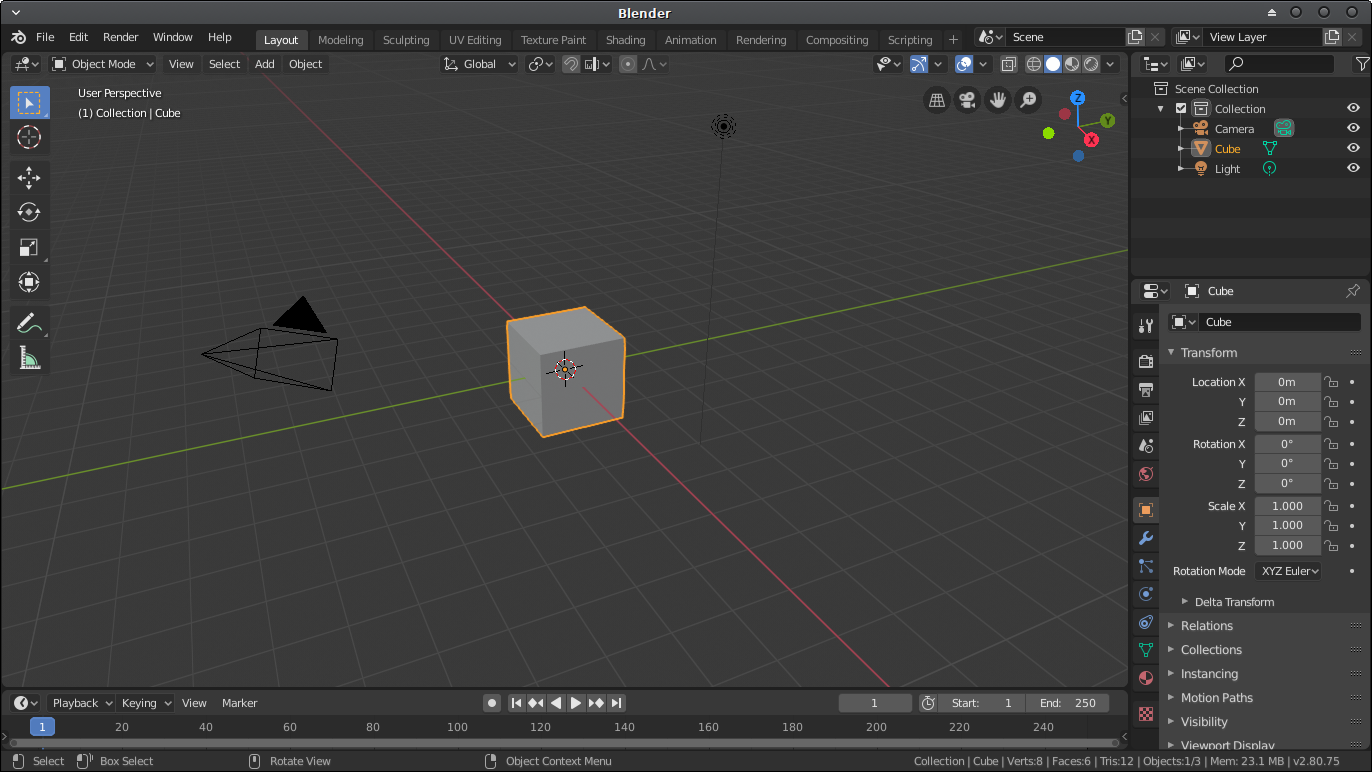
\includegraphics[width=6.5in]{img/methodology_generatingData_blender_startscreen.png}
	\caption{Blender interface after startup. The default scene features a grey cube, a camera (left of the cube) and a light source (black dot and circle positioned on the top right of the cube).}
	\label{pic:methodology_generatingData_blender_startscreen}
\end{figure}

The authors decided to extensively use the scripting function in their work. One example of a Python script, that can be executed in blender is the following code:

\begin{lstlisting}[language=python]
import bpy

# Selects all cubes and deletes them
bpy.ops.object.select_all(action='DESELECT')
bpy.ops.object.select_by_type(type='MESH')
bpy.ops.object.delete()

# Adds a new cube
bpy.ops.mesh.primitive_cube_add(size=3, enter_editmode=False, location=(4, 2, 0))

# Adds a new material representing the colour red
bpy.ops.material.new()
material = bpy.data.materials[-1]
material.name = 'Red'
material.diffuse_color = (0.8, 0.1, 0.1, 1)

# Apply material onto the newly created cube object
bpy.context.active_object.data.materials.append(material)
\end{lstlisting}

This code first clears the scene from other meshes (because running the script twice would place the new cube inside the old cube). Then it adds a new mesh in form of a cube at the given location. Next we want to add some color to the cube. For this to work a material is needed, which is basically a specification of how the surface of the object will look like. Advanced materials can represent raw or reflective surfaces, but in order to keep it simple this material will just represent a red surface (represented in red/green/blue/alpha channels ranging from 0.0 (for 0) to 1.0 (for 255)). Lastly the created material is applied to the object. The final result can be seen below:

\begin{figure}[h!]
	\centering
	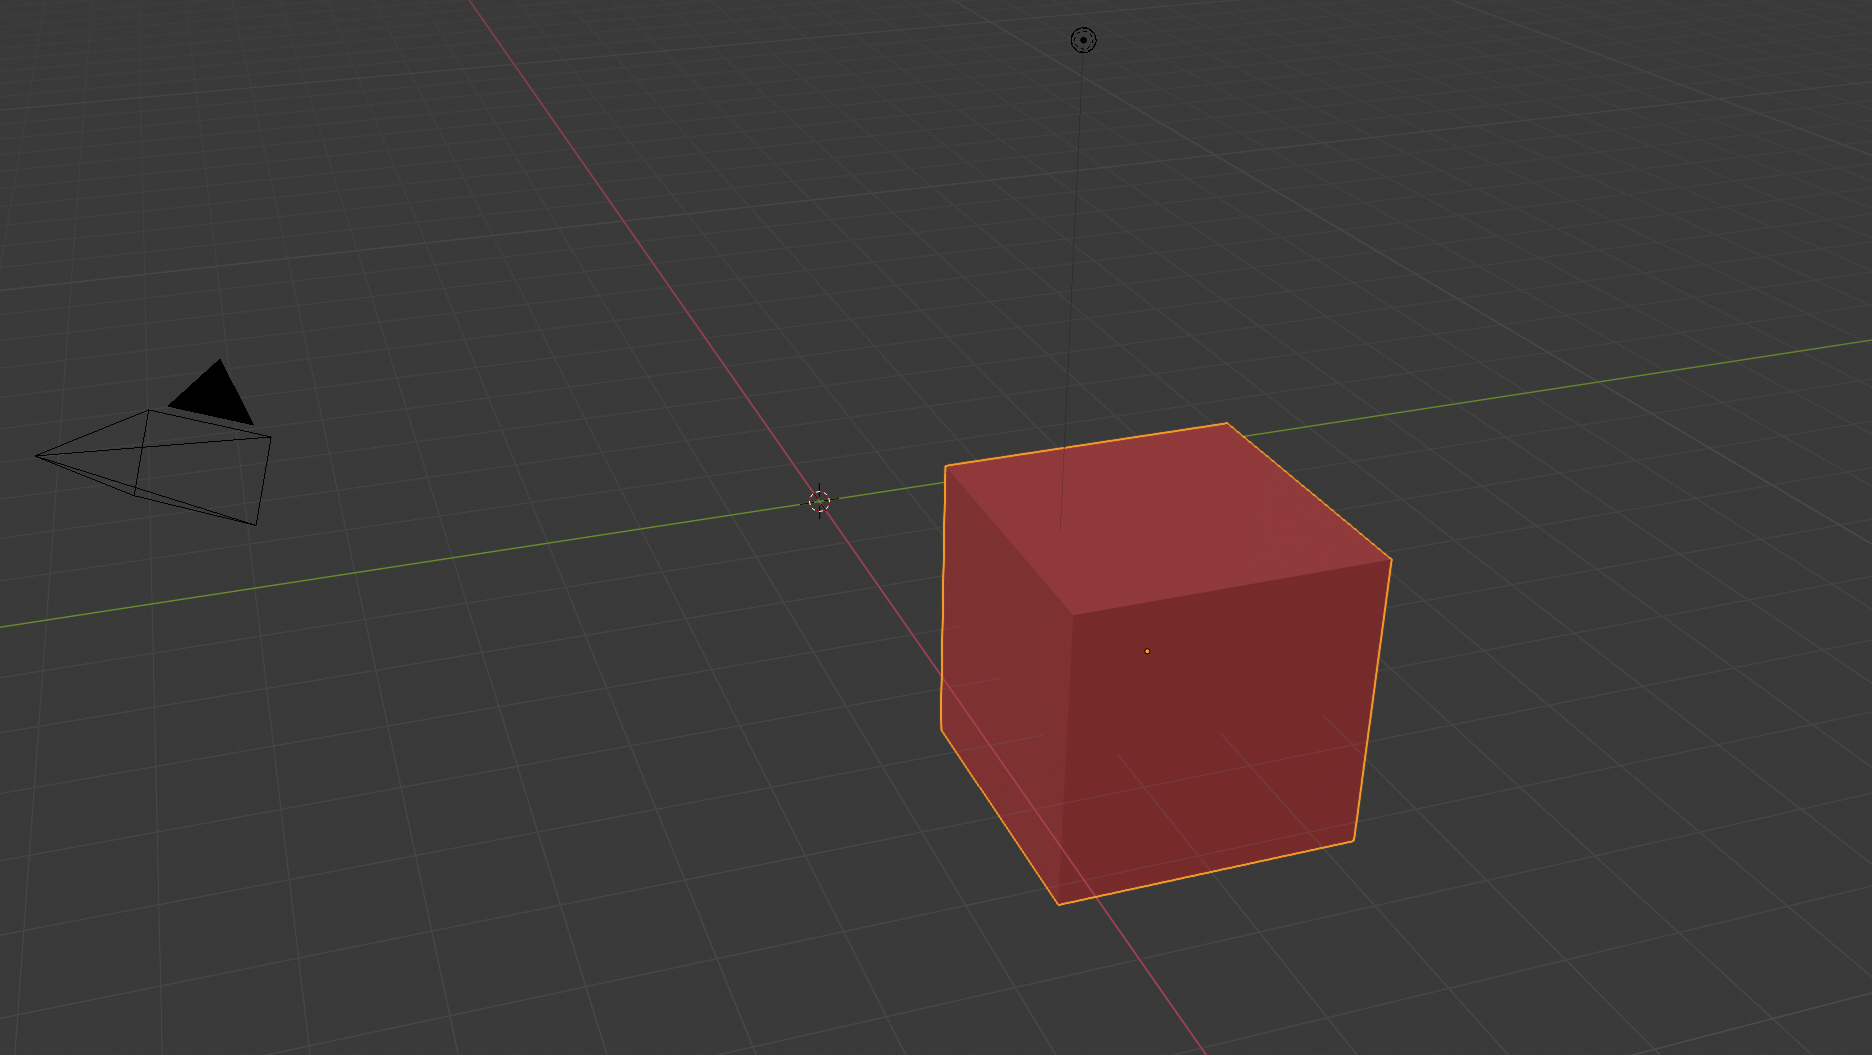
\includegraphics[width=6.5in]{img/methodology_generatingData_blender_exampleScriptResult.png}
	\caption{Result of the above code. The default cube is deleted, a new one is added with a red material and translated via the 'location' argument.).}
	\label{pic:methodology_generatingData_blender_exampleScriptResult}
\end{figure}

Using similar Python scripts the authors will generate the image data necessary as well as perform the calculation of the distance which will be specified as the correct values to train the neural network on.

\section{Image preprocessing}
After the test images have been rendered with the help of Blender some image preprocessing is required. For example the machine learning component of this project should take two images as an input. To simplify the input the two images will simply be placed next to each other to form a new image twice as wide as the original images. This process is visualized in Figure~\ref{pic:methodology_imagePreprocessing_imageMerge}. Other preprocessing measures that have to be taken are downscaling the image, as to not have too many weights in the first layer of the neural network.

\begin{figure}[h!]
	\centering
	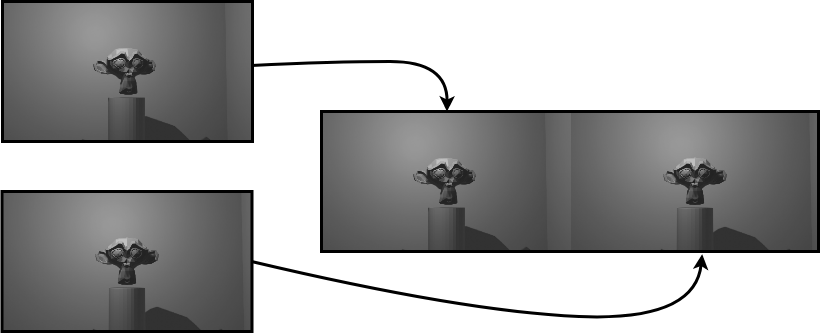
\includegraphics[width=6.5in]{img/methodology_imagePreprocessing_imageMerge.png}
	\caption{Two greyscale renders showing the same object from two different camera positions in Blender are merged into one picture which can be feed into the neural network component.}
	\label{pic:methodology_imagePreprocessing_imageMerge}
\end{figure}

Additionally, the authors decided to experiment if manipulating these test images further would result in differences of distance perception by the neural network or if they would speed up or slow down the learning phase. These manipulations are done using OpenCV and Python3. OpenCV provides many image manipulation tools. For this project the authors chose the following methods of image manipulation:

\begin{table}[h!]
	\begin{tabular}{|l|l|}
		\hline
		\bfseries Name & \bfseries Description \\
		\hline
		Greyscale & A greyscale image is an image with only one value for the red, green and \\
		& blue colour channels, resulting in different shades of grey instead of usual \\
		& colours. \\
		\hline
		Resolution & Resolution refers to the number of pixels placed in each dimension \\
		& (width and height). \\
		\hline
		Cropping & When cropping an image an unwanted part located at the peripheral areas \\
		& of the image is removed. \\
		\hline
		Saturated & Saturated images feature stronger colours, which makes them easier to \\
		& distinguish from another. \\
		\hline
		Brightness & Brightening images can make colours harder to distinguish from another. \\
		& Additionally it can lead to the same problems encountered in overexposed \\
		& images, such as part of the image being completely white and therefore not \\
		& providing any information. \\
		\hline
	\end{tabular}
\end{table}


\section{Neural Network}
A Neural Network consists of nodes, each receiving some input values as well as some weights associated to each input value and outputs some output value. The calculation returning the output value is relatively simple. Many of these nodes form what is called a layer. A vanilla Neural Network consists of multiple layers, where each node receives all output values of all nodes in the previous layer as an input. A visualization of a Neural Network can be seen in Figure~\ref{pic:methodology_neuralNetwork_visualizationOfANN}. By manipulating the weights associated to each input value the network can learn to solve some given task.

\begin{figure}[h!]
	\centering
	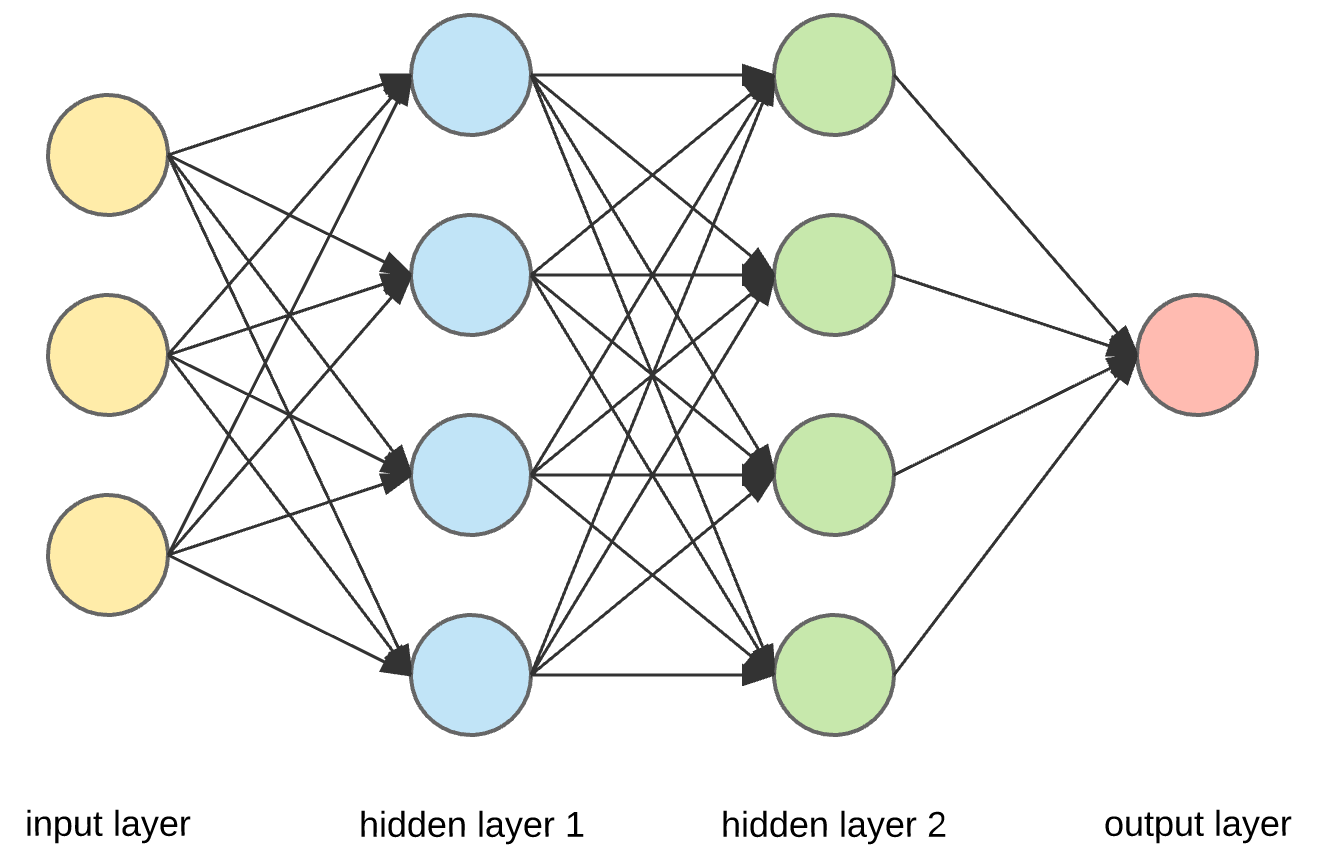
\includegraphics[width=4.5in]{img/methodology_neuralNetwork_visualizationOfANN.png}
	\caption{Depiction af a vanilla Neural Network. Each circle represents a node and the arrows show the flow of information. All nodes on the same level are collectively called a layer.}
	\label{pic:methodology_neuralNetwork_visualizationOfANN}
\end{figure}

\subsection{Convolutional Neural Network}
One of the disadvantages of Neural Networks is that they need huge amounts of data in order to optimize the values of all weights. Therefore a modified version of Neural Networks was invented. Convolutional Neural Networks simplify the optimization of the weights by stating that some weights are shared between multiple connections between nodes. This results in fewer weights having to be optimized. Additionally Convolutional Neural Networks contribute to the fact that often problems require to perform similar actions in multiple parts of the input data, e.g. search for edges in all sections of an image.

\begin{figure}[h!]
	\centering
	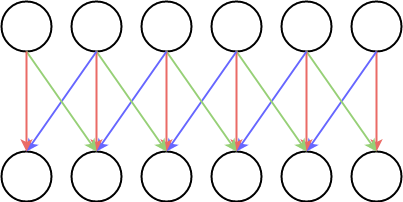
\includegraphics[width=1.5in]{img/methodology_neuralNetwork_visualizationOfACNN.png}
	\caption{Segment of a Convolutional Neural Network. In comparison to a vanilla Neural Network each node is only connected to its closest neighbours. Additionally all arrows connected to another node in the same relative position (same colour) have the same weight attached.}
	\label{pic:methodology_neuralNetwork_visualizationOfACNN}
\end{figure}

\section{Neural Network Implementations}
The authors decided to use a software framework called TensorFlow for the first implementation of the neural network. This has the following two advantages: using Tensorflow allows for a low effort proof of concept and it makes testing out different configurations (e.g. number of hidden layers or filters in image preprocessing) of the neural network easier.

After it has been shown that the challenge of detecting the distance to an object can be solved using machine learning, the authors plan on implementing a neural network in C++ on their own. The knowledge gained in the TensorFlow implementation will be used in the C++ implementation, which hopefully will make the work less time consuming.

\section{TensorFlow}
As machine learning has gained popularity in recent years the demand for applicable frameworks grew. One of the most popular is called TensorFlow. It was developed by Google for internal use and was published under the Apache License 2.0 on the \nth{9} of November 2015.

TensorFlow supports APIs for Python, C, C++, Go, Java, JavaScript and Swift.
Due to its popularity third party APIs for C\#, R, Scala, Rust and many more were developed.

Its use cases reach from categorizing handwritten digits to YouTube video recommendations, one of the many applications Google use it for.

Tom Hope et al. describe TensorFlow as a software framework for numerical computations based on dataflow graphs \footcite[page 6]{Hope_Learning_TensorFlow}.

\subsection{Computation graph}
To compute a value using TensorFlow a computation graph has to be constructed. In this graph each node corresponds to an operation, such as subtraction or division. By connecting these nodes via edges the output of one node can be fed as input into another node. One example of such a computation graph can be seen in Figure~\ref{pic:methodology_tensorflow_computationGraph}.

\begin{figure}[h!]
	\centering
	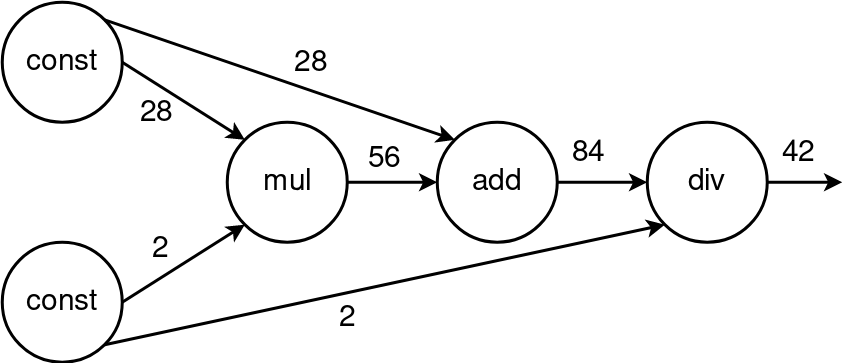
\includegraphics[width=4.5in]{img/methodology_tensorflow_computationGraph.png}
	\caption{Each node represents an operation, where $const$ stands for a constant value, $add$ for addition, $mul$ for multiplication and $div$ for division. Edges, represented by arrows, connect nodes. The information shared between the nodes is described by the numbers written next to the edges. This computational graph calculates the result of the arithmetic expression $(28 * 2) + 28 / 2$.}
	\label{pic:methodology_tensorflow_computationGraph}
\end{figure}

The implementation of the computation graph, shown in Figure~\ref{pic:methodology_tensorflow_computationGraph}, in Python could look as follows:

\begin{lstlisting}[language=python]
import tensorflow as tf

a = tf.constant(28)
b = tf.constant(2)

c = tf.multiply(a, b)
d = tf.add(a, c)
e = tf.divide(d, b)

with tf.Session() as sess:
out = sess.run(e)

print(out)
\end{lstlisting}

The first line specifies that the TensorFlow functionality should be imported. Line 3 and 4 define the two constant values and assigns them the values 28 and 2 respectively. In line 6 to 8 the other nodes of the graph are specified. E.g. in line 6 a new node, named $c$, is created and the output of node $a$ and node $b$ are connected as its input. To perform the calculation described by the graph a new session is created in line 10. Finally the output of the graph (node $e$) is specified in line 11, the result is calculated and printed in line 13.

TensorFlow allows for another way of specifying a graph with these arithmetic operations:

\begin{lstlisting}[language=python]
import tensorflow as tf

a = tf.constant(28)
b = tf.constant(2)

e = (a * b + a) / b

with tf.Session() as sess:
out = sess.run(e)

print(out)
\end{lstlisting}

This code is equivalent to the first one, but uses syntactic sugar to shorten line 6 to 8 in the first code block into line 6. At this point it should be noted that while it might look like it line 6 does not calculate anything. It simply describes how the computational graph should look. The answer (42) is calculated in the session in line 9.

Using the same principle, but different functions TensorFlow allows the creation of complex Neural Networks in a simple fashion.

\subsection{Alternatives to Tensorflow}
TensorFlow offers some abstraction libraries, such as Keras. As some code snippets of are used very frequently and with only slight variation when implementing a Neural Network, Keras offers these code blocks as predefined functions, making development easier for ``standard'' use cases.

For example Keras provides several different layers, that can be used to put together a Neural Network. Table~\ref{tab:methodology_tensorflow_alternativesToTensorflow_kerasLayers} describes some of the available layers.

\begin{table}[h!]
	\begin{center}
		\begin{tabular}{| l | l |}
			\hline
			\bfseries Name & \bfseries Description \\
			\hline
			Dense & regular densely connected layer \\
			\hline
			Activation & Applies an activation function to an output \\
			\hline
			Dropout & Applies Dropout to the input \\
			\hline
			Flatten & Flattens the input down to shape \verb|(None, <number of elements>)| \\
			\hline
			Conv1D & 1D convolution layer (e.g. temporal convolution)  \\
			\hline
			MaxPooling1D & Max pooling operation for temporal data \\
			\hline
			LocallyConnected1D & Locally-connected layer for 1D inputs \\
			\hline
			SimpleRNN & Fully-connected RNN where the output is to be fed back to input \\
			\hline
		\end{tabular}
		\label{tab:methodology_tensorflow_alternativesToTensorflow_kerasLayers}
		\caption{Short description of layers available in Keras, that can be used to assemble a Neural Network, with little effort\footcite{kerasDocumentation}.}
	\end{center}
\end{table}


[INFO: Abstraction libraries such as Keras and TF-Slim offer simplified  high-level  access  to  the  "LEGO  bricks"  in  the  lower-level  library,  helping  to streamline the construction of the dataflow graphs, training them, and running inference. \footcite[page 7]{Hope_Learning_TensorFlow}]

\begin{table}[h!]
\begin{center}
	\begin{tabular}{| l | l | l | l | l |}
		\hline
		\bfseries & \bfseries Open Source & \bfseries Actively & \bfseries Parallelization & \bfseries Interface \\
		& & \bfseries developed & & \\
		\hline
		\bfseries TensorFlow & Yes & Yes & Yes & Python, C, C++, \\
		& & & & Go, Java, JavaScript, \\
		& & & & Swift, R, Julia \\
		\hline
		\bfseries Keras & Yes & Yes & Yes & Python \\
		\hline
		\bfseries PyTorch & Yes & Yes & Yes & Python, C++ \\
		\hline
		\bfseries Torch & Yes & No & Yes & Lua, LuaJIT, C, \\
		& & & & C++, OpenGL \\
		\hline
		\bfseries Wolfram & No & Yes & Yes & Wolfram Language \\
		\bfseries Mathematica & & & & \\
		\hline
	\end{tabular}
	\label{tab:methodology_tensorflow_alternativesToTensorflow_comparision}
\end{center}
\end{table}

[+ warum verwenden wir ausgerechnet Tenserflow]

\filbreak
